\documentclass[]{beamer}
\usepackage{amssymb,amsmath}
\usepackage{fixltx2e}
\usepackage{lmodern}
\usepackage{tikz}
\IfFileExists{upquote.sty}{\usepackage{upquote}}{}
\IfFileExists{microtype.sty}{\usepackage{microtype}}{}

\usetheme{Warsaw}
\usecolortheme{crane}
\usebackgroundtemplate{%
\tikz\node[opacity=0.2] {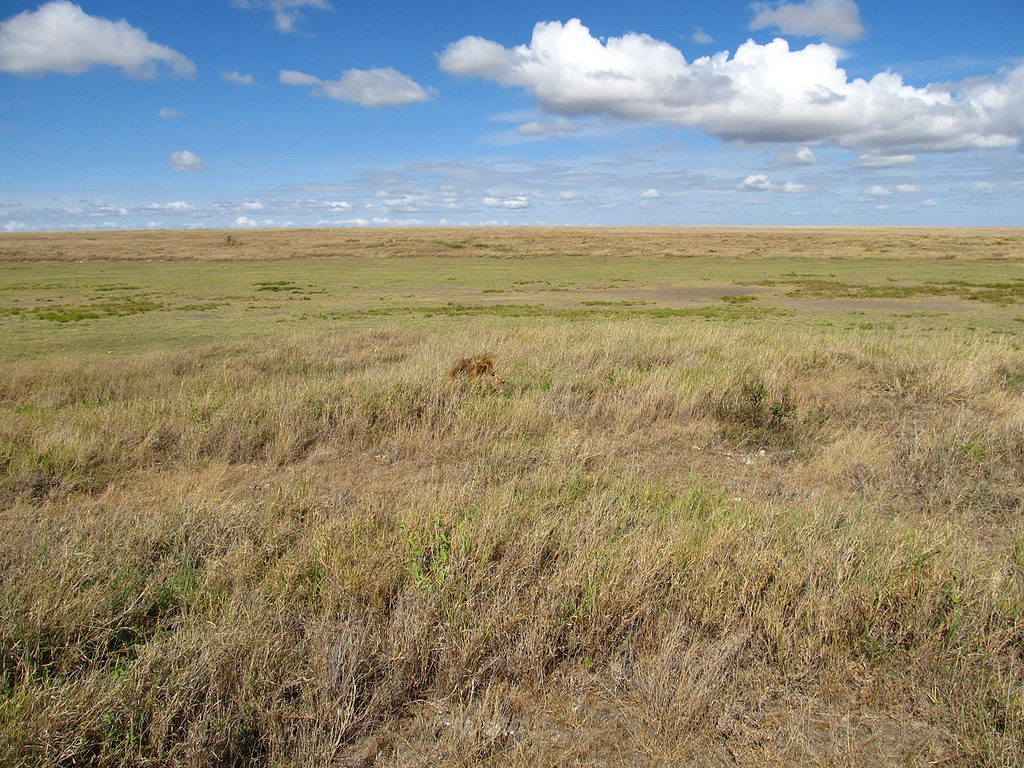
\includegraphics[height=\paperheight,width=\paperwidth]{images/Serengeti_background.jpg}};}

\setbeamercolor{mycolor}{fg=red,bg=olive}

\defbeamertemplate*{footline}{shadow theme}{%
\leavevmode%
\hbox{\begin{beamercolorbox}[wd=.5\paperwidth,ht=2.5ex,dp=1.125ex,leftskip=.3cm plus1fil,rightskip=.3cm]{author in head/foot}%
    \usebeamerfont{author in head/foot}\hfill\insertshortauthor
\end{beamercolorbox}%

\begin{beamercolorbox}[wd=.5\paperwidth,ht=2.5ex,dp=1.125ex,leftskip=.3cm,rightskip=.3cm plus1fil]{title in head/foot}%
    \usebeamerfont{title in head/foot}\insertshorttitle\hfill%
\insertframenumber\,/\,\inserttotalframenumber
\end{beamercolorbox}}%
\vskip0pt%
}

\setlength{\parindent}{0pt}
\setlength{\parskip}{6pt plus 2pt minus 1pt}
\setlength{\emergencystretch}{3em}  % prevent overfull lines
\setcounter{secnumdepth}{0}

\title{Stochasticity and Evolution in Food Webs}
\author{Giulio Dalla Riva\\
\tiny{gvd16@uclive.ac.nz}\\
}
\date{  {\tiny Biomathematical Research Centre\\
  University of Canterbury\\
     gvdr.github.io\\
     \vskip 0.5cm
  }
Granada Seminar June 16, 2015}

\begin{document}
\frame{\titlepage
\addtocounter{framenumber}{-1}}

\begin{frame}{Why?}

\centering
\begin{tabular}{|c|c|}\hline
Evolution & Ecology \\\hline\hline
Phylogeny & Food Web \\
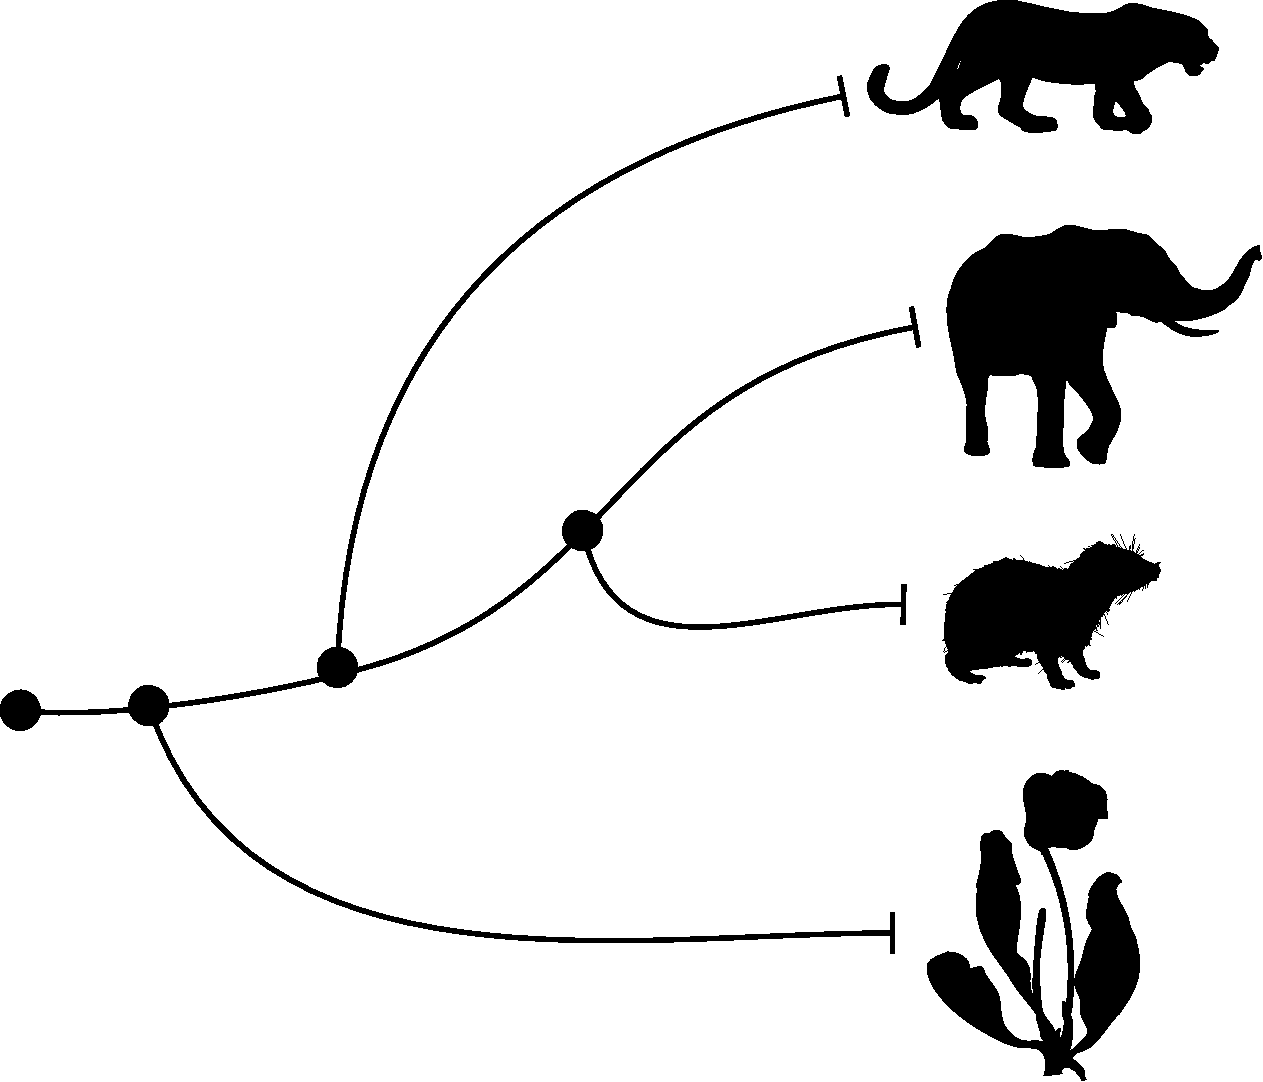
\includegraphics[width=0.4 \textwidth]{images/small_phylo.pdf} & 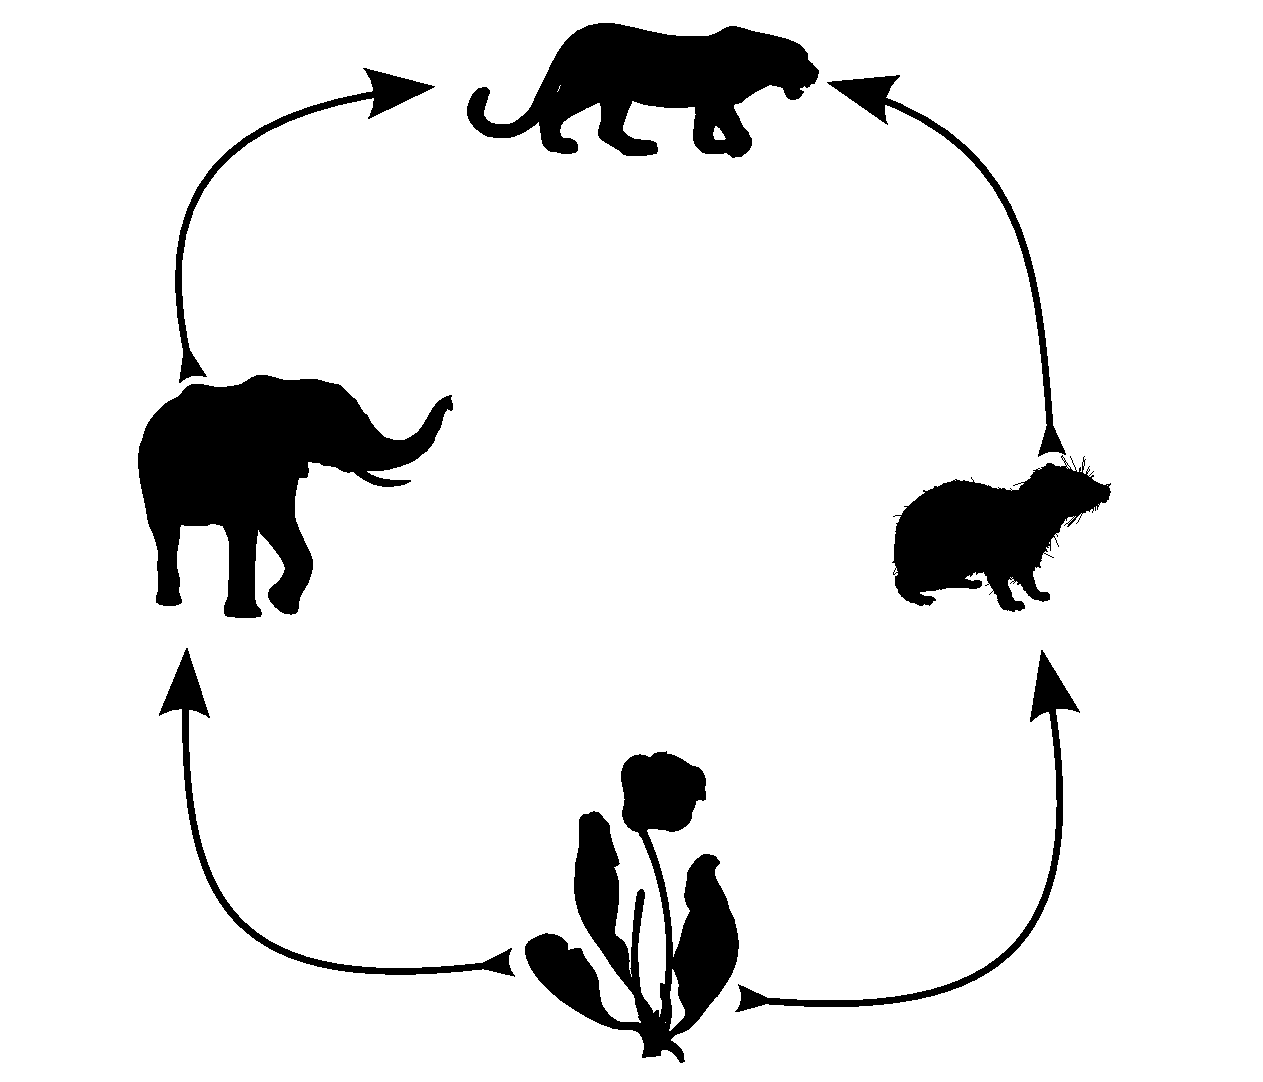
\includegraphics[width=0.4 \textwidth]{images/small_fw.pdf} \\ \hline
\end{tabular}

\end{frame}

\begin{frame}{What?}

\centering
The backbones of a food web exhibits an Evolutionary signal.

\centering
\begin{tabular}{cc}
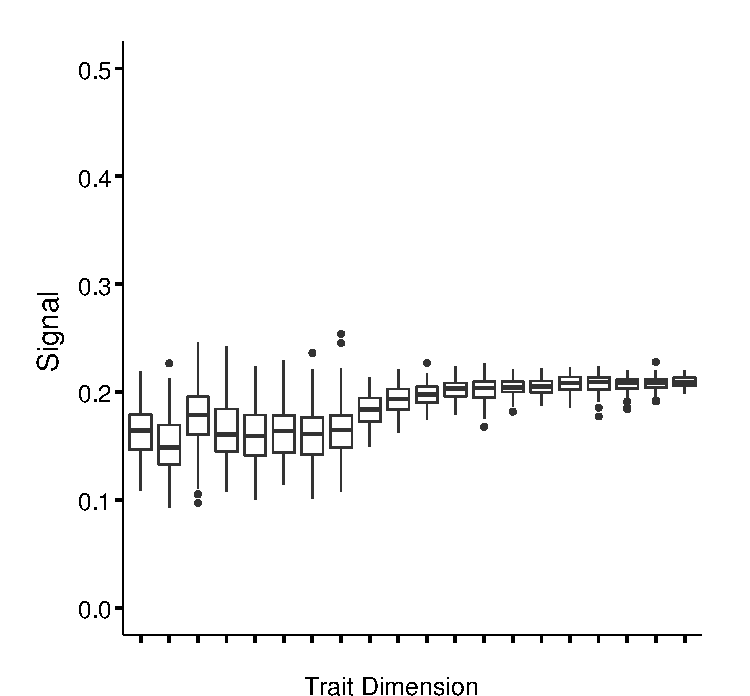
\includegraphics[width=0.47\linewidth]{images/psig.pdf} & 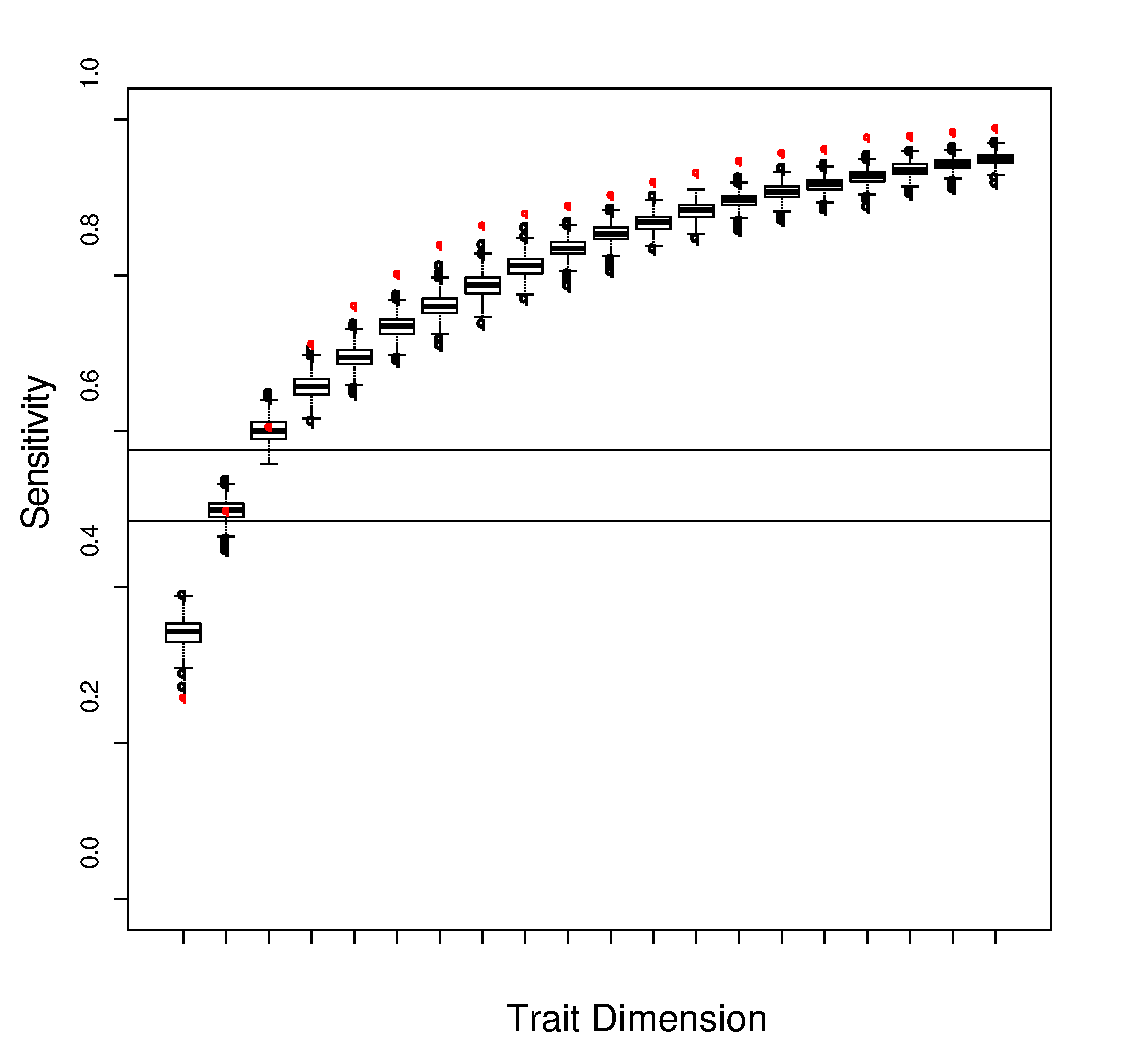
\includegraphics[width=0.47 \linewidth]{images/sens.pdf}\\
{\tiny Phylogenetic signal} & {\tiny Model sensitivity}
\end{tabular}

\footnote{From gvdr \& Stouffer, in press}

\end{frame}

\begin{frame}{How?}

\begin{itemize}[<+->]
\centering
\item
Random Dot Product Graphs

  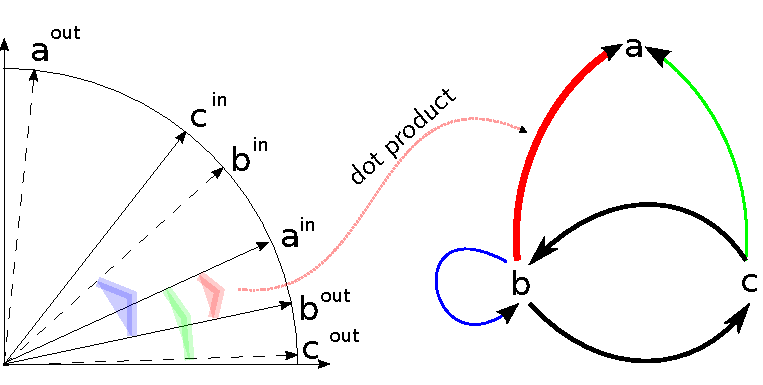
\includegraphics[width=0.8\linewidth]{images/RDPGmodel.pdf}

\footnote{From gvdr \& Stouffer, in press}

\item
Expected vs.~Observed trait distribution
  \begin{equation*}
    \textrm{vcv}\left( \mathbb{T} | \tau, \mbox{model} \right) \mbox{ vs. } \textrm{vcv}\left(\mathbb{T}\right)
  \end{equation*}

\end{itemize}

\end{frame}

\begin{frame}{So what?}

\begin{itemize}[<+->]
\itemsep1pt\parskip0pt\parsep0pt
\item
  There is phylogenetic signal\\
  {\tiny p-values anybody?}
\item
  It is quite weak\\
  {\tiny $20\% ~ 30\%$ of variation explained}
\item
  It saturates with dimensionality\\
  {\tiny $d \in \left\{2, \dots , 8 \right\}$}
\item
  $\therefore$ ``fine wirings'' may be deceiving
\item
What about the null model?

{\em
{\scriptsize Although species evolve and diversify in a complex network of species interactions, current models of diversification typically ignore species interactions. [These models] do not allow analysing the effect of species interactions on diversification.

H\'{e}l\`{e}ne Morlon - \textrm{Ecology Letters} (2014) \textbf{17}: 508-525}
}
\end{itemize}

\end{frame}

\begin{frame}{And now?}

  Spoiler: An ecological aware evolutionary model is (almost) there:
  
  \small yes, I am looking at you, Ornstein and Uhlenbeck $\dots$

\end{frame}

\begin{frame}{Who?}

\begin{centering}
\small{
Joint work with  
Daniel B. Stouffer (University of Canterbury)

Many thanks to  
Mike Steel; Carey Priebe; A. Mooers', D.B. Stouffer's \& J. Tylianakis' lab; ...

Funds by the Allan Wilson Centre for Molecular Ecology and Evolution.}

\centering
  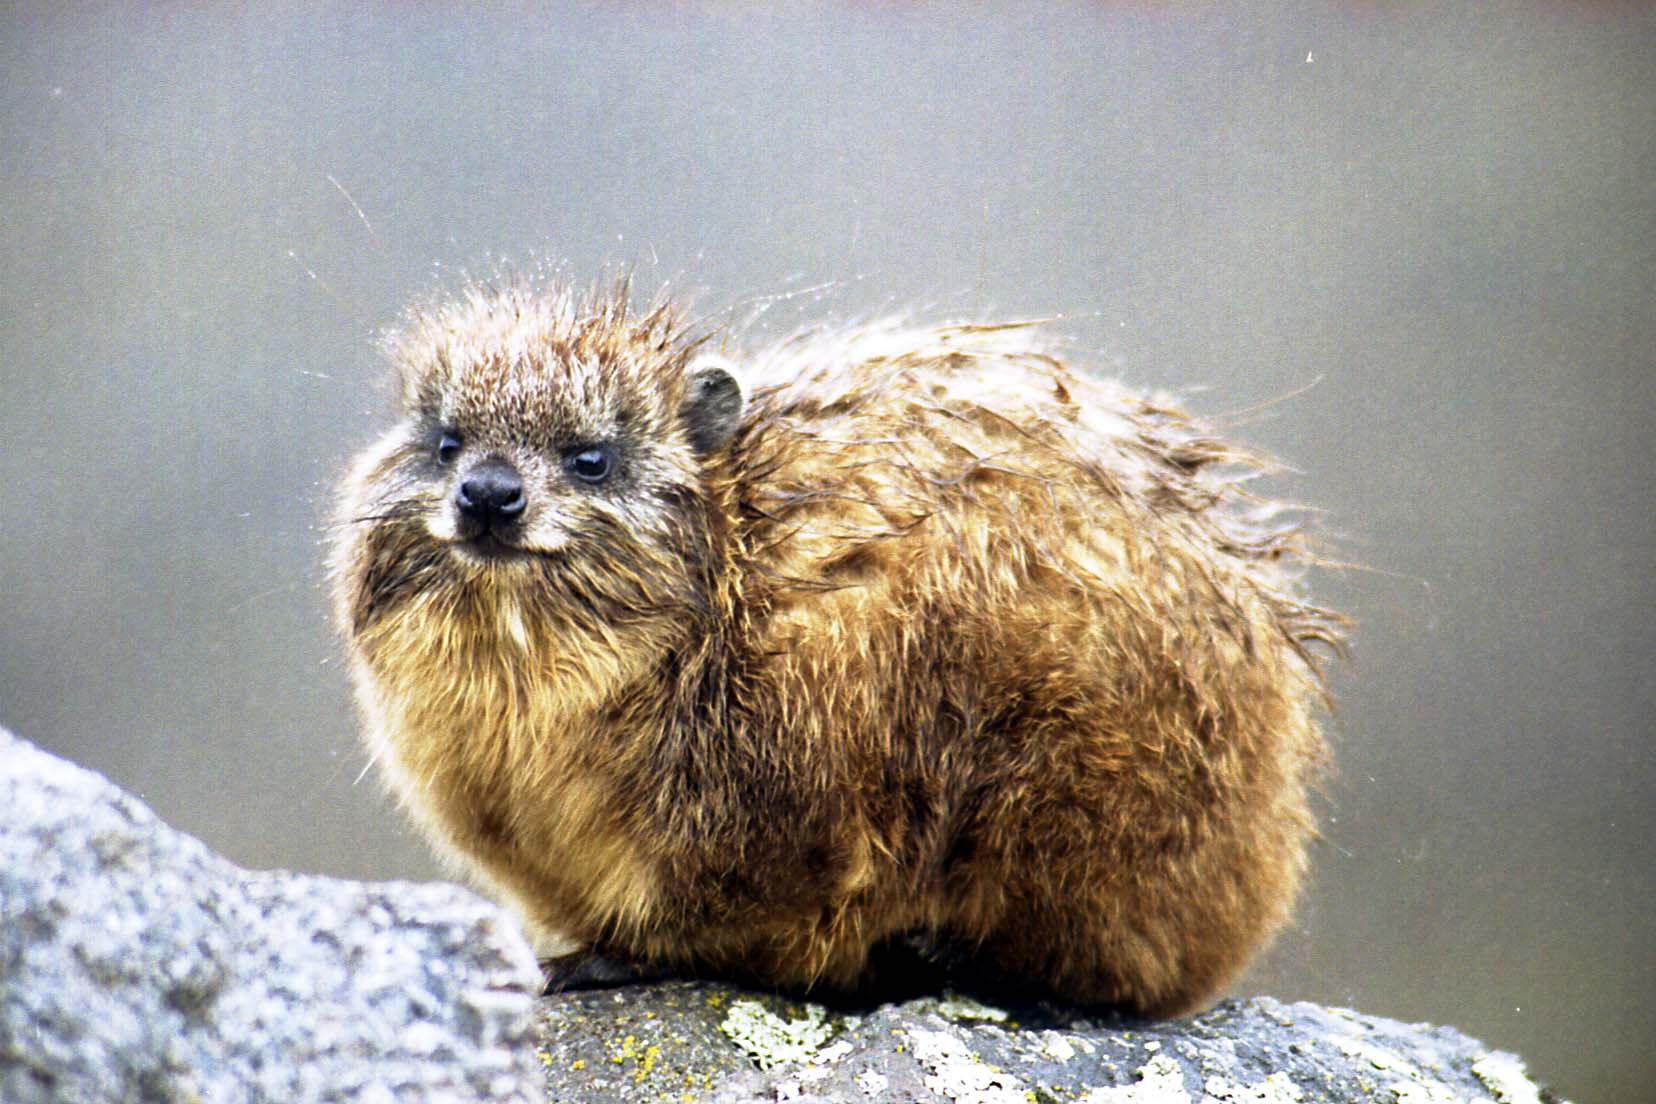
\includegraphics[width=0.4\linewidth]{images/hyrax.jpg}

\small{By the way, I'm looking for a postdoc.\\ gvd16@uclive.ac.nz - gvdr.github.io}

\end{centering}

\end{frame}

\end{document}
